\section{Introduction}
\label{sec:intro}
\vspace{-1mm}

\begin{figure*}[t]
    \centering
    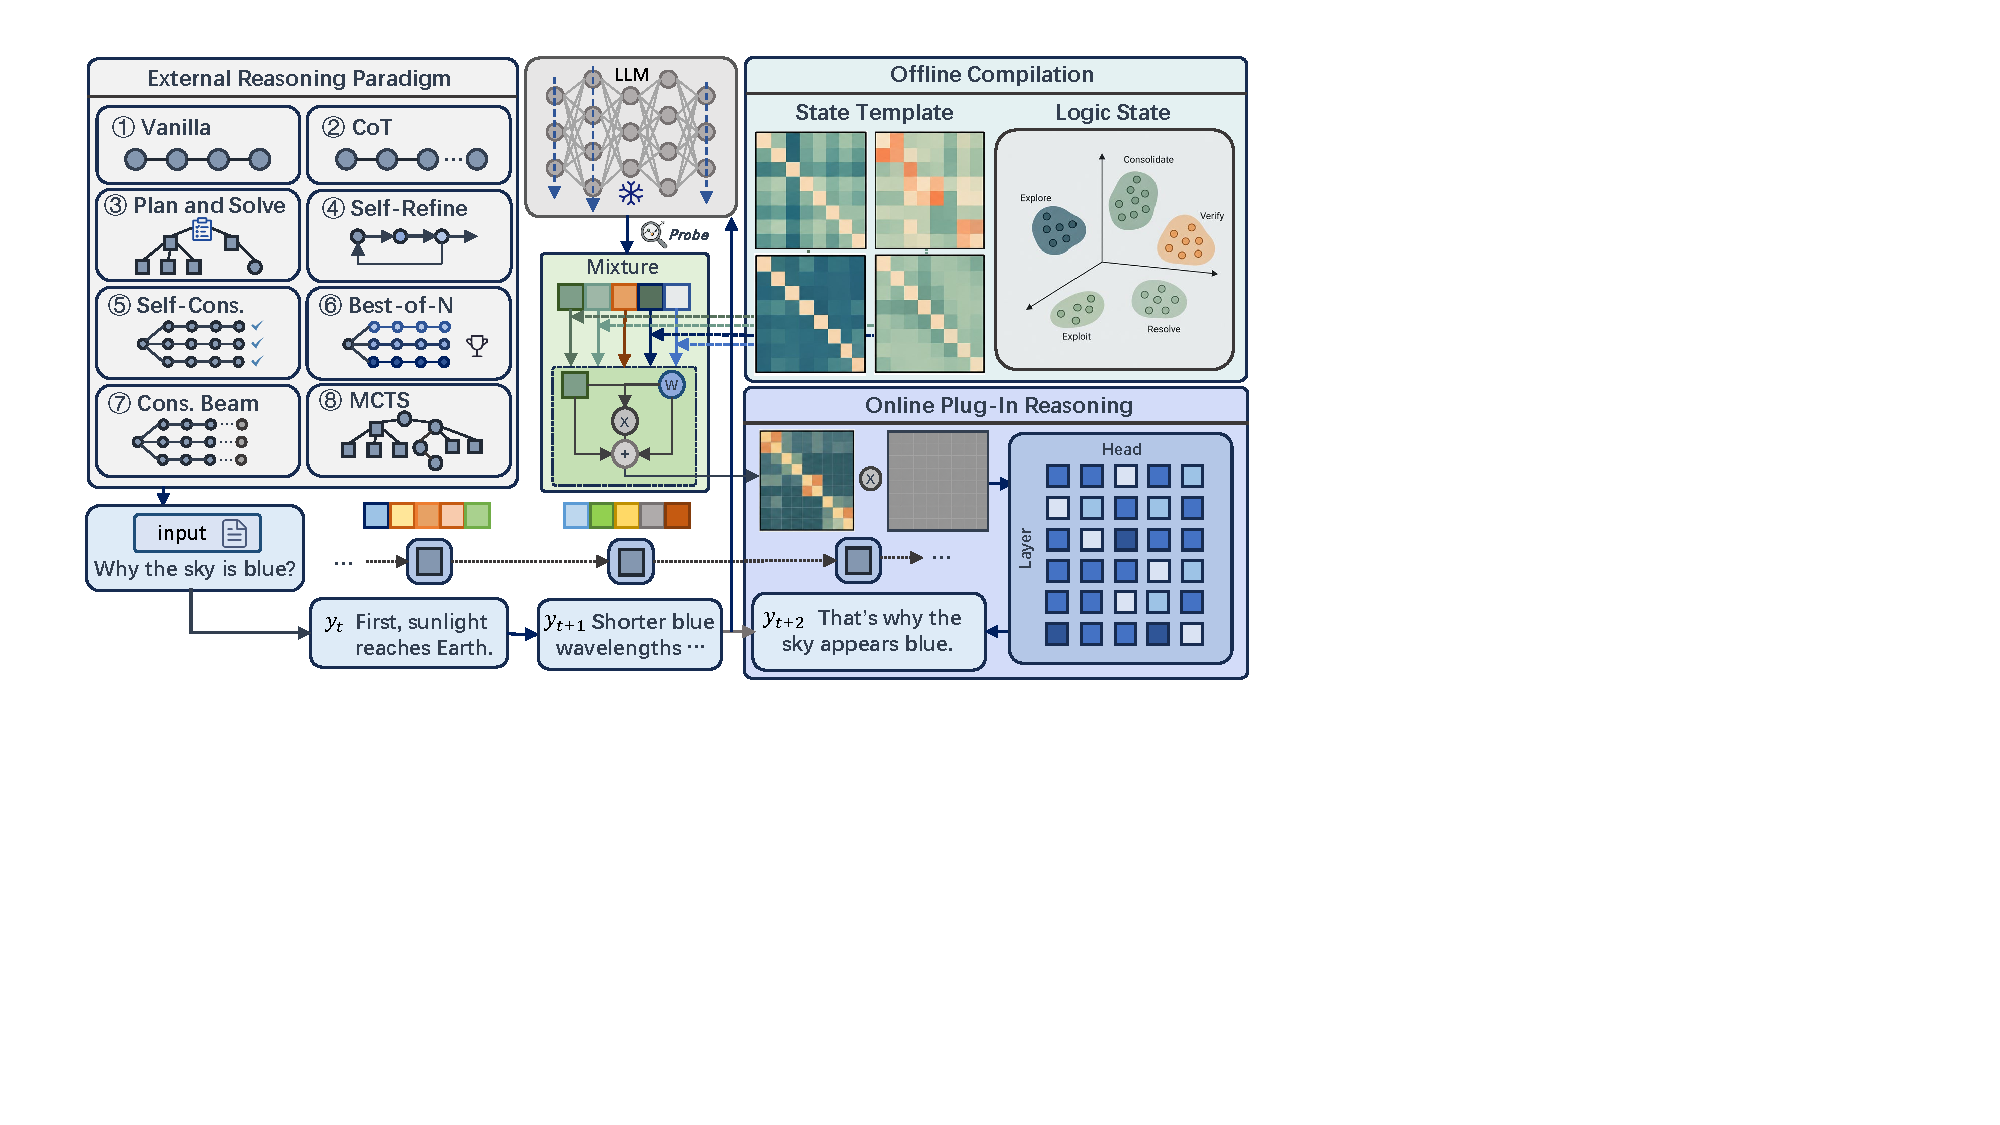
\includegraphics[width=\linewidth]{figs/intro_main.pdf}
    \vspace{-4mm}
    \caption{
    LoTR as plug-and-play reasoning through logic-conditioned internal pathway routing.
    }
    \vspace{-7mm}
    \label{fig:intro_main}
\end{figure*}

Reasoning has become a primary way to improve the problem-solving ability of Large Language Models (LLMs) \citep{chen2023pot,gao2023pal,yao2023react,zhou2023least}.
Recent progress largely comes from extensive \emph{reasoning paradigms} that prescribe \emph{external reasoning strategies}, such as structured step decomposition \citep{wang2023plan,wei2022chain}, iterative revision \citep{madaan2023selfrefine}, planning \citep{wang2023plan,yao2023tree}, and search-and-sampling \citep{brown2024llmmonkeys,snell2025scaling,wang2023selfconsistency}. 
Although differing in form, these paradigms follow the same basic mechanism: push the model toward better reasoning performance by specifying stronger external procedures \citep{chen2023pot,gao2023pal} or by spending more computation on sampling, branching, or verification \citep{lightman2024verify,xie2024mcts}.
This mechanism brings high effectiveness but still leaves an important complementary dimension less examined.
Specifically, the model executes reasoning through fixed \emph{internal computation pathways} with reasoning strategies prescribed, rarely asking whether those internal pathways are well matched to the \emph{dynamic reasoning logic} induced by the strategy.
This mismatch may leave part of the benefit of external reasoning strategies unrealized, especially when different reasoning steps require different internal modes of execution.


This limitation motivates us to examine the model's \emph{internal logic states} as latent execution modes that evolve throughout reasoning, and to use them to guide reasoning through more suitable internal computation pathways.
Prior studies on model internals \citep{zou2023representationengineering} and reasoning interpretability \citep{zhang2025reasoningmodels} suggest that reasoning is internally non-uniform, with different strategies \citep{hao2024coconut,he2026beyondcot} and even different steps within the same strategy \citep{sun2026trajectories} inducing distinct logic states.
Meanwhile, analyses of transformer computation suggest that attention heads are differentiated contributors to reasoning-time information transfer, collectively shaping the pathways determining how the reasoning is carried out \citep{michel2019sixteen,olsson2022induction,voita2019analyzing}. 
Together, these observations suggest that internal logic states and head-level differences exist, yet existing reasoning paradigms rarely couple the two: they prescribe \emph{which strategy} to follow externally, but do not decide \emph{which internal pathway} to use internally under dynamic reasoning logic.
Therefore, these motivations raise a question: \emph{Can dynamic logic states be coupled with internal pathway routing to enable reasoning paradigms to execute more effectively?}

We propose \textbf{Logic-of-Thought Routing (LoTR)}, a lightweight plug-and-play reasoning module that strengthens existing reasoning paradigms through \emph{logic-conditioned internal pathway routing}.
LoTR builds a compact view of dynamic logic states from the model's internal information transfer and links these states to stable patterns of attention-head pathways. 
During reasoning, a lightweight linear probe infers the current logic-state mixture from the ongoing step, and the model is then softly routed through the pathway most suitable for the current reasoning logic. 
In this way, LoTR complements existing reasoning paradigms with prescribed external strategies by making their internal execution more adaptive to the logic that each reasoning step actually requires.

Across 3 backbones, 8 benchmarks, and 8 reasoning paradigms, LoTR improves paradigm-averaged accuracy by 16.67\%, 4.25\%, and 4.94\% on Llama-3.1-8B, Qwen2.5-14B, and Mixtral-8$\times$7B, respectively. 
Overall, this yields a 7.93\% relative accuracy gain with only +3.18\% generated tokens and +6.93\% end-to-end latency. 
The trade-off remains favorable across backbones: LoTR reduces latency by 10.76\% on Llama and 12.15\% on Mixtral, and uses 2.28\% fewer tokens on Qwen. 
These results show that LoTR shifts the accuracy--efficiency frontier of existing reasoning paradigms, suggesting that reasoning can be improved not only by expanding external search or sampling, but also by routing each step through an internal pathway matched to its current logic.